%!TEX root = ../../csuthesis_main.tex
\chapter{绪论}

本文主要致力于研究面向智慧交通场景的多目标跟踪算法和评测。

\section{研究背景和研究意义}

\subsection{研究背景}

研究背景:
随着人工智能技术的发展,多目标跟踪算法在智慧交通领域取得了显著进展。这些算法能够实时监测和分析交通流量,为交通管理提供了新的解决方案。传统的交通监控系统往往面临效率低下、成本高昂等问题,而基于多目标跟踪算法的智能交通系统能够提供更加智能、高效的服务,提升交通运行效率和公共安全\cite{dollar2016unified}。

本研究旨在设计并开发一个基于大语言模型的营销客服对话系统,以实现以下目标:提高交通监控效率,降低交通管理成本,提升公共安全和交通效率,为交通规划和政策制定提供数据支持,推动智慧交通技术的发展,促进跨学科融合,应对复杂交通场景挑战。总体上来讲,面向智慧交通场景的多目标跟踪算法和评测的研究,不仅涉及算法的开发和优化,还包括算法在实际交通场景中的应用和评测。这些研究对于提高交通管理的智能化水平、增强公共安全、推动智慧城市建设等方面具有重要的意义\cite{wojke2017simple}。


\begin{figure}[htbp] % 可以是h(here),t(top),b(bottom),p(page of floats)
	\centering
	\includegraphics[width=1\textwidth]{car1} % 假设图片文件名为car.pdf或car.png等,位于当前工作目录
	\caption{汽车} % 图片标题
	\label{fig:car1} % 用于引用的标签
\end{figure}



\subsection{研究意义}

研究意义:
提高交通安全和效率,利于智能驾驶辅助技术的发展,构建智能交通监控系统,解决复杂场景下的跟踪问题,应对实时性和鲁棒性挑战,促进智能交通技术的发展,促进跨摄像头跟踪和数据关联。面向智慧交通场景的多目标跟踪算法和评测的研究,对于提升交通管理的智能化水平、增强交通安全、促进智能交通技术的发展等方面具有重要的意义和价值。\cite{yu2020deep}


\begin{figure}[htbp] % 可以是h(here),t(top),b(bottom),p(page of floats)
	\centering
	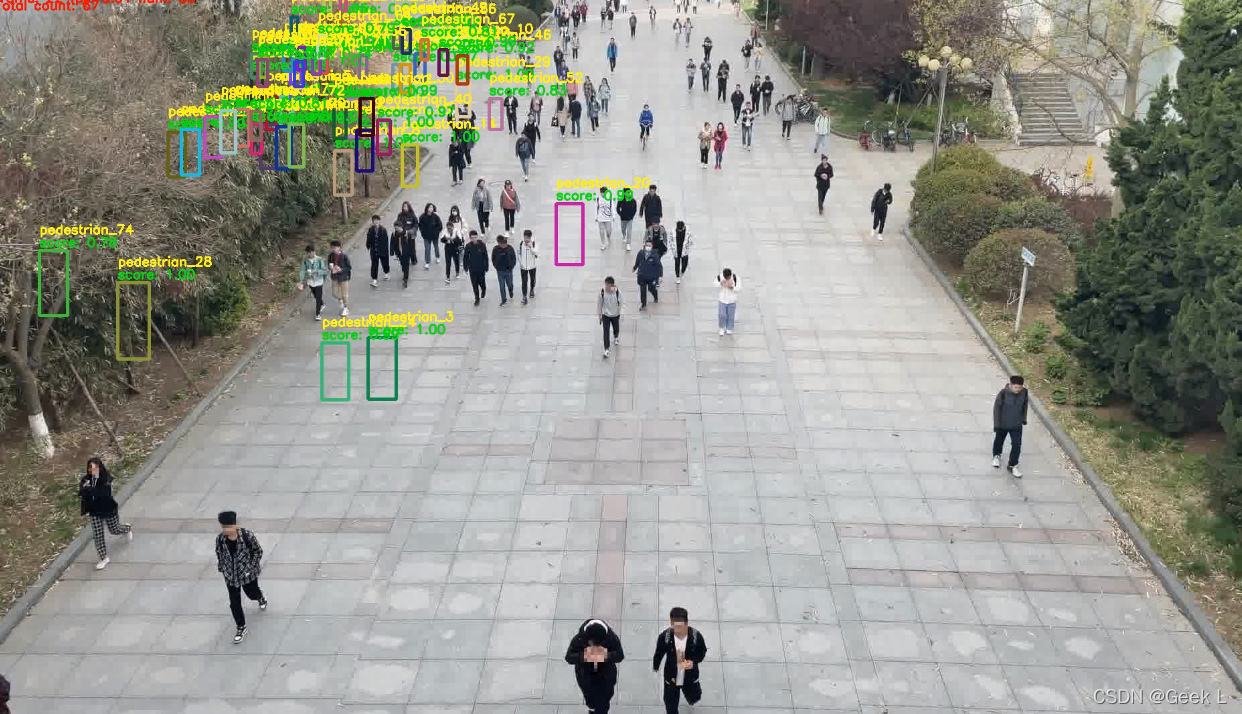
\includegraphics[width=1\textwidth]{people} % 假设图片文件名为car.pdf或car.png等,位于当前工作目录
	\caption{检测} % 图片标题
	\label{fig:people} % 用于引用的标签
\end{figure}


\section{国内外研究动态}

\subsection{国外研究动态}

深度学习特征提取的新突破:研究者们提出了多种基于深度学习的特征提取技术,如ZippyPoint,该技术通过混合精度离散化加速兴趣点检测、描述和匹配,显著提高了网络运行速度、描述符匹配速度和3D模型大小,实现了至少一个数量级的改进。

基于动态规划的检测前跟踪(DP-TBD)算法:研究者们对基于动态规划的检测前跟踪算法进行了系统研究,这种算法在硬件上易实现,计算量和存储量相对较小,显示出在多目标跟踪领域的潜力\cite{lynch2017introduction}。

Transformer在Re-ID中的应用:基于Transformer的Re-ID研究正在改变长期由卷积神经网络(CNN)主导的格局,不断刷新性能记录,取得重大突破。研究人员全面回顾了Transformer在Re-ID中日益增长的应用研究,并深入分析了Transformer的优势。

优化YOLOv4算法的低空无人机检测与跟踪:研究者们提出了基于优化YOLOv4的低空无人机检测与跟踪方法,结合了检测技术和跟踪算法,以实现低空无人机的动态检测\cite{一种行人与自动驾驶车辆的交互博弈均衡策略探究方法}。

多目标多摄像头跟踪系统(MTMCT):OCMCTrack框架的提出,该框架通过引入新的匹配级联来动态重新评估轨迹分配,最小化在线跟踪器常犯的误报关联\cite{}。

无监督行人Re-ID的研究:中科院的研究团队在顶刊TIP 2023上发表了题为“Rethinking Unsupervised Person Re-ID”的文章,深入探讨了无监督行人Re-ID的问题。

\begin{figure}[htbp] % 可以是h(here),t(top),b(bottom),p(page of floats)
	\centering
	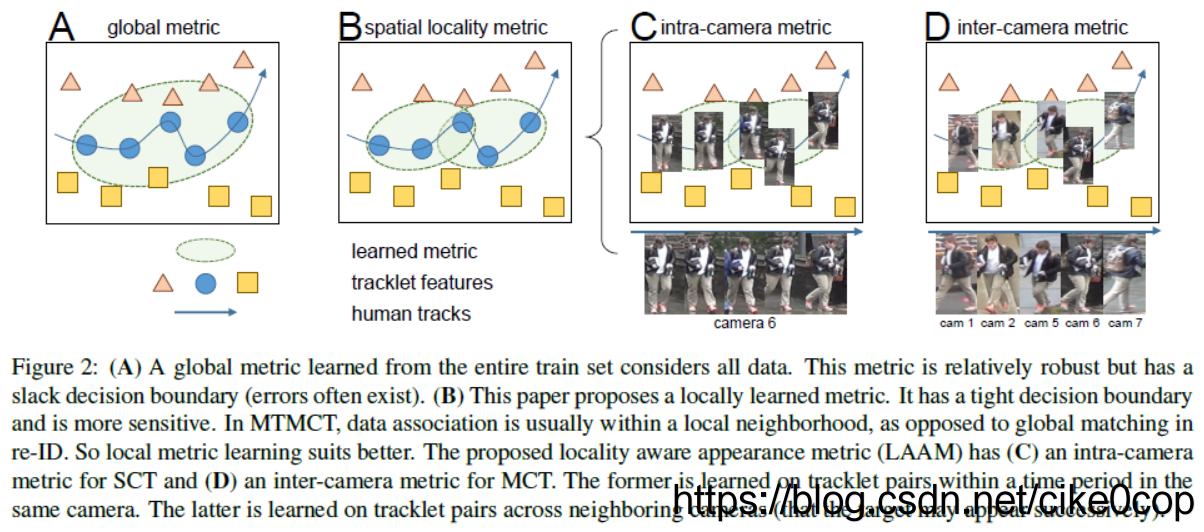
\includegraphics[width=1\textwidth]{people3} % 假设图片文件名为car.pdf或car.png等,位于当前工作目录
	\caption{国外研究} % 图片标题
	\label{fig:people3} % 用于引用的标签
\end{figure}


\subsection{国内研究动态}

跨摄像头多目标跟踪方法综述:国内研究人员对跨摄像头多目标跟踪方法进行了综述,探讨了多种技术路线和算法进展,包括基于深度学习的特征提取和目标跟踪技术\cite{zhou2020tracking}。

中国特色轨迹数据集构建:清华大学苏州汽车研究院和江苏智能网联汽车创新中心致力于建设中国特色轨迹数据集,从真实道路交通数据中提取各类车辆、行人等轨迹信息,构建了包含多种道路类型的轨迹数据集Mirror-Traffic。这些数据集被广泛应用于智能驾驶、交通模拟等领域的模型开发与验证工作\cite{bewley2016simple}。

视频交通监控系统发展趋势:《2024至2030年中国视频交通监控系统数据监测研究报告》深入探讨了中国视频交通监控系统的未来发展趋势,指出随着城市化进程的加速与智能交通管理需求的增长,视频交通监控系统将更加智能化、集成化\cite{韩炳庆 2018 智能交通场景中的多目标跟踪算法研究}。

中国典型驾驶场景库i-Scenario:中国汽研发布了中国典型驾驶场景库i-Scenario及仿真测试全平台工具链,该场景库涵盖标准法规、人工经验数据、中国交通事故数据和自然驾驶数据四大数据源,可应用于MIL、SIL、HIL等虚拟仿真系统。

基于自适应特征融合的目标跟踪算法:国内研究者提出了一种基于自适应特征融合的相关滤波跟踪算法,该算法采用方向梯度直方图特征和卷积神经网络来对目标进行信息构建,并利用特征响应的峰值旁瓣比和旁瓣值占比自适应地确定融合系数,以预测目标位置。

行人再识别技术研究进展:国内研究人员总结了遮挡行人再识别、无监督行人再识别、虚拟数据生成、域泛化行人再识别等热点方向的前沿进展,并展望了行人再识别技术的发展趋势\cite{kalman1960new}。

\section{研究内容与方法}

应用深度学习技术,特别是卷积神经网络(CNN),以自动学习目标特征。
探索自适应权重的三元组损失函数和难例挖掘技术,以优化多目标多相机追踪(MTMCT)和行人再识别(Re-ID)性能\cite{choi2020multiple}。
研究基于元数据辅助重识别(MA-ReID)和基于轨迹的相机链接模型(TCLM)。

\begin{figure}[htbp] % 可以是h(here),t(top),b(bottom),p(page of floats)
	\centering
	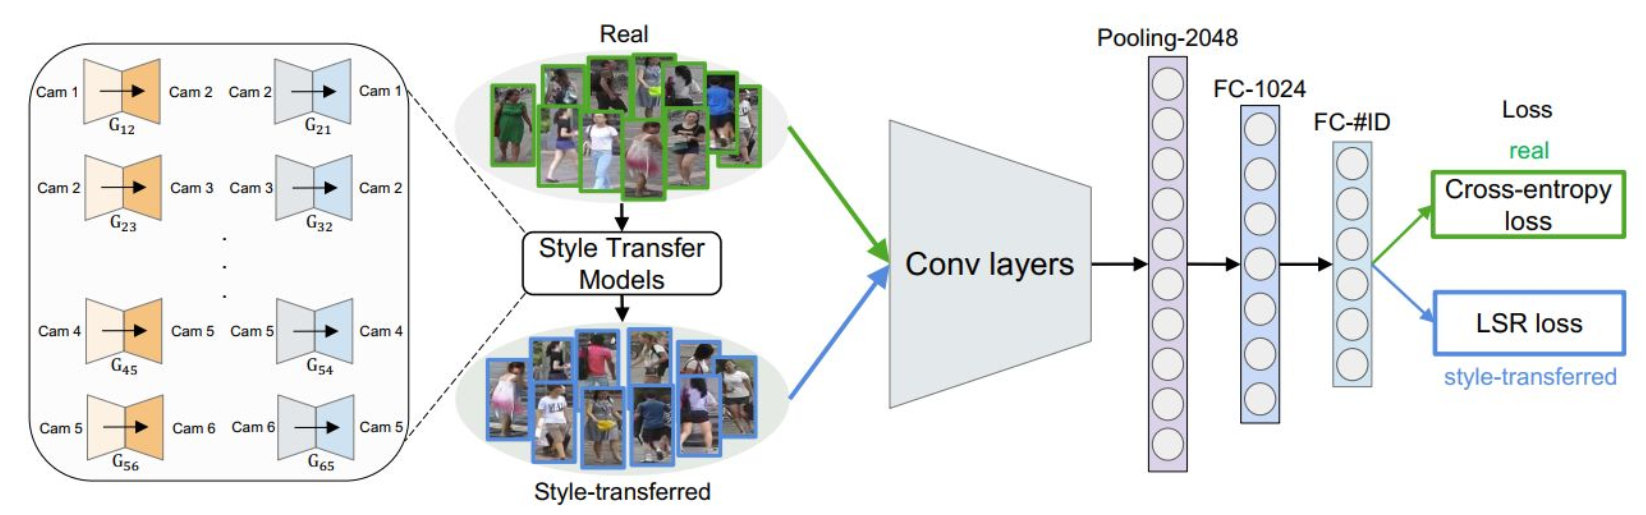
\includegraphics[width=1.0\textwidth]{people2} % 假设图片文件名为car.pdf或car.png等,位于当前工作目录
	\caption{研究方法} % 图片标题
	\label{fig:people2} % 用于引用的标签
\end{figure}

